% Optical Response Classification of Carbon Allotropes
% via Electronic Delocalization and Effective Conduction Dimensionality
% Draft v4 — March 2026

\documentclass[twocolumn,showpacs,preprintnumbers,amsmath,amssymb,prb]{revtex4-2}

\usepackage{graphicx}
\usepackage{amsmath}
\usepackage{amssymb}
\usepackage{bm}
\usepackage{hyperref}
\usepackage{booktabs}
\usepackage{xcolor}

% Figure path
\graphicspath{{../simulation/figures/}}

\begin{document}

\preprint{Draft v4}

\title{Optical Response Classification of Carbon Allotropes \\
via Electronic Delocalization and Effective Conduction Dimensionality}

\author{K.~Miyauchi}
\affiliation{Independent Researcher}

\date{\today}

\begin{abstract}
The macroscopic optical appearance of materials---transparent, colored,
black, or lustrous---cannot be fully classified by the band gap alone.
Both metals and graphite possess a vanishing band gap, yet the former
exhibits metallic luster while the latter appears black with cleavage-plane
gloss.

We propose that the essence of luster is the preservation of photon phase
coherence at interfaces, and that its microscopic condition reduces to the
\emph{freedom of constituent particles}. In metals, delocalized electrons
enable collective response; in liquids, molecular mobility ensures
self-smoothing interfaces. Both mechanisms preserve incident-photon phase
relations, yielding specular reflection.

To rigorously test this idea, we restrict the scope to solid-state
electronic systems and introduce two variables: an effective delocalization
index~$\delta$ and an effective conduction dimensionality~$D_\mathrm{eff}$.
Using five carbon allotropes (diamond, C$_{60}$, SWCNT, graphene, graphite)
and hexagonal boron nitride (h-BN) as a control, we collect three
$\delta$-proxy indicators (the $\pi$-band width, the inverse effective mass,
and the band gap) from the published literature. We demonstrate that
(1)~pairwise correlations among the three proxies are statistically
significant (Pearson $r = 0.70$--$0.89$, Spearman $\rho = 0.83$--$0.88$),
supporting the existence of an overarching variable~$\delta$;
(2)~a decision tree based on $E_g$ and $D_\mathrm{eff}$ classifies all
seven materials into the correct optical-response category with 100\%
accuracy; and
(3)~h-BN, despite sharing the layered sp$^2$ structure of graphite, is
transparent---direct evidence that $\delta$ is an independent variable.

The framework does not replace band-gap theory but extends it: $E_g$
determines \emph{at which energy} the response occurs, while
$D_\mathrm{eff}$ determines its \emph{directionality}. The concept of
particle freedom~($\delta$) motivated the introduction of
$D_\mathrm{eff}$; independent verification of $\delta$ as a measurable
variable in liquid and interfacial systems is proposed as a future
target.
\end{abstract}

\maketitle

% =====================================================================
\section{Introduction}
% =====================================================================

\subsection{The luster question: photon coherence preservation}

Liquids universally exhibit luster. So do metals. Although the microscopic
origins differ---polarization response versus free-electron response---the
macroscopic phenomenon is the same: incident photons are re-emitted at the
interface with their mutual phase relationships intact. A mirror image
forms precisely because the phase coherence of the reflected photon
ensemble is preserved.

Conventional physics explains metallic luster via the Drude model and
liquid reflection via the Fresnel equations, treating them as separate
phenomena. No unified framework derives both from a single underlying
principle.

\subsection{Particle freedom and the quantum barrier}

We propose that the condition for photon coherence preservation at an
interface reduces to the \emph{freedom of constituent particles}.

A material interface acts as a quantum barrier for incident photons. The
character of this barrier determines the optical response:

\begin{itemize}
  \item \textbf{Localized particles} ($\delta$ low): each scatterer
    responds independently; the re-emitted phases are randomized. The
    barrier is incoherent. Result: diffuse scattering (transparent or
    white).
  \item \textbf{Delocalized particles} ($\delta$ high): scatterers
    respond collectively and coherently; re-emitted phases are aligned.
    The barrier is coherent. Result: specular reflection (luster).
\end{itemize}

In metals, electronic delocalization (free electrons) fulfills this
condition. In liquids, molecular delocalization (fluidity) guarantees
interface self-smoothing, fulfilling the same condition through a
different mechanism.

\subsection{Scope: proof of concept in solid carbon}

In liquids, both the electronic degree of freedom ($\delta_\mathrm{elec}$)
and the nuclear degree of freedom ($\delta_\mathrm{nuc}$) vary
simultaneously, making their effects difficult to disentangle. In solids,
$\delta_\mathrm{nuc}$ is frozen, isolating the effect of
$\delta_\mathrm{elec}$.

The present work is a \textbf{proof of concept}: we test the overarching
hypothesis in the most controlled setting available. Carbon allotropes are
chosen because a single element spans the full range of optical
appearances---transparent (diamond), colored (C$_{60}$, semiconducting
SWCNTs), black (graphite), and lustrous (graphite cleavage
plane)---allowing us to vary $\delta$ and $D_\mathrm{eff}$ while
eliminating elemental composition as a confounding factor.

Extension to liquid, interfacial, and catalytic systems is a natural
consequence of the framework and is proposed as a target for future,
independent experimental verification.

\subsection{Gap in the existing classification}

The macroscopic optical appearance of materials falls into four broad
categories: transparent (diamond), colored (ruby), black (graphite),
and metallic luster (silver). Existing theories explain each category
individually, but no unified predictive framework based on a common set
of classification variables has been established.

In particular, the following questions lack a unified answer:
\begin{itemize}
  \item Why do metals and graphite, both having a vanishing band gap,
    differ so dramatically in optical response?
  \item Why are h-BN and graphite---both layered sp$^2$
    networks---white and black, respectively?
  \item Why does a single element (carbon) cover all four optical
    categories?
\end{itemize}

% =====================================================================
\section{Framework}
\label{sec:framework}
% =====================================================================

\subsection{Causal structure}

At the most general level, the freedom of constituent particles
($\delta$) determines whether an interface acts as a coherent or
incoherent quantum barrier for photons. In solid-state electronic
systems, this reduces to the product of two variables:

\begin{equation}
  \text{Optical response} = f\!\left(\delta_\mathrm{elec},\;
  D_\mathrm{eff}\right),
  \label{eq:causal}
\end{equation}

\noindent where $\delta_\mathrm{elec}$ quantifies the degree of
electronic delocalization and $D_\mathrm{eff}$ quantifies the effective
dimensionality of electronic conduction. The concept of particle
freedom~($\delta$) motivated the introduction of $D_\mathrm{eff}$ as a
classification variable: if the optical response depends on how freely
particles can move, one must specify not only \emph{whether} they can
move (encoded in~$E_g$) but also \emph{in how many directions}
(encoded in~$D_\mathrm{eff}$).

The central insight is that $E_g$ alone provides an incomplete mapping
from electronic structure to optical response. Adding $D_\mathrm{eff}$
completes the mapping. The measurable classification variables are
$E_g$ and $D_\mathrm{eff}$; $\delta$ serves as the physical intuition
that unifies them and whose independent verification in liquid and
interfacial systems is proposed as a future target.

\subsection{Effective delocalization index $\delta$: operational definition}

$\delta$ is not a single physical quantity but an overarching variable
whose existence is inferred from the mutual consistency of several proxy
indicators:

\begin{table}[h]
\caption{Candidate proxy indicators for $\delta$.}
\label{tab:delta_proxies}
\begin{ruledtabular}
\begin{tabular}{lll}
  Indicator & Definition & Advantage \\
  \hline
  $\pi$-band width $W_\pi$ & Full energy width of & Direct comparison \\
   & the $\pi$ band (eV) & among sp$^2$ systems \\
  Inverse effective & Curvature of $E(k)$ & Defined for all \\
  mass $1/m^*$ & at band edge & materials \\
  IPR & $\sum_i |\psi_i|^4$ & Direct measure of \\
   & & delocalization \\
  Wannier spread & $\langle r^2 \rangle - \langle r \rangle^2$ &
  Physically transparent \\
\end{tabular}
\end{ruledtabular}
\end{table}

Our strategy is to show that multiple proxies yield the same ordering
across materials, thereby supporting the existence of an overarching
variable $\delta$ without requiring a unique definition.

\subsection{Effective conduction dimensionality $D_\mathrm{eff}$:
  operational definition}
\label{sec:Deff}

$D_\mathrm{eff}$ is defined as the \textbf{effective rank of the
group-velocity tensor} evaluated for electronic states near the Fermi
level or band edges:

\begin{equation}
  D_\mathrm{eff}
    = \operatorname{rank}_\mathrm{eff}\!\bigl(\langle v_\alpha\, v_\beta \rangle\bigr),
  \label{eq:Deff}
\end{equation}

\noindent where $v_\alpha = \hbar^{-1}\,\partial E(\bm{k})/\partial k_\alpha$
is the band group velocity and the average is taken over states within
an energy window $\Delta E$ of the band edge (we adopt
$\Delta E = 1$~eV). The effective rank counts the number of principal
directions along which $\langle v_\alpha\, v_\beta \rangle$ exceeds a
threshold $v_\mathrm{thresh}^2$ (we use
$v_\mathrm{thresh} = 10^{4}$~m\,s$^{-1}$, corresponding to a
bandwidth $W \approx 0.5$~eV over a typical Brillouin-zone extent).
Equivalently, $D_\mathrm{eff}$ equals the number of principal
directions with significant band dispersion, but defined through the
velocity tensor rather than bandwidths, making it directly computable
from DFT band structures or Wannier-interpolated Hamiltonians without
reference to any optical measurement.

This definition is \emph{purely electronic and structural}: it depends
only on the band dispersion $E(\bm{k})$ and therefore avoids
circularity with the optical response it is used to classify.

\begin{table}[h]
\caption{Crystallographic vs.\ effective conduction dimensionality.}
\label{tab:Deff}
\begin{ruledtabular}
\begin{tabular}{lccc}
  Material & Crystal dim. & $D_\mathrm{eff}$ & Rationale \\
  \hline
  Diamond      & 3D     & 0 & $E_g = 5.47$~eV; no states \\
               &        &   & in visible window \\
  C$_{60}$ fcc & 3D     & 0 & Intermolecular $t \sim 30$~meV; \\
               &        &   & $W \approx 0.5$~eV \\
  SWCNT        & 1D     & 1 & Axial dispersion only \\
  Graphene/    & 2D/3D  & 2 & In-plane $W \approx 9$~eV \\
  \quad Graphite &      &   & $\gg$ interlayer $\gamma_1 \approx 0.4$~eV \\
  Metals       & 3D     & 3 & Isotropic conduction \\
  h-BN         & 2D     & 0 & $E_g = 5.95$~eV; no states \\
               &        &   & in visible window \\
\end{tabular}
\end{ruledtabular}
\end{table}

Note that h-BN possesses a 2D crystal structure with in-plane band
dispersion ($W_\pi \approx 2.4$~eV), but because its band gap
($5.95$~eV) places all $\pi$-band states far outside the visible-energy
window, $D_\mathrm{eff} = 0$. The distinction between crystallographic
dimensionality and $D_\mathrm{eff}$ is essential to the framework.

\subsection{Decision tree for optical response classification}
\label{sec:tree}

The two variables $E_g$ and $D_\mathrm{eff}$ define a decision tree:

\begin{enumerate}
  \item $E_g > E_\mathrm{vis} \approx 3.1$~eV? \\
    $\to$ \textbf{Yes}: Transparent (no electronic response in the
    visible range). \\
    $\to$ \textbf{No}: proceed to step~2.
  \item $E_g > 0$? \\
    $\to$ \textbf{Yes}: Colored (selective absorption). \\
    $\to$ \textbf{No} ($E_g \approx 0$): proceed to step~3.
  \item Classification by $D_\mathrm{eff}$: \\
    $D_\mathrm{eff} = 1$: Black with weak luster (1D metallic). \\
    $D_\mathrm{eff} = 2$: Black with cleavage-plane gloss (2D metallic). \\
    $D_\mathrm{eff} = 3$: Full metallic luster (3D metallic).
\end{enumerate}

\subsection{Second-order corrections}

The two-variable framework captures the dominant trends. Known
second-order effects include:
\begin{itemize}
  \item \textbf{Polarity/ionicity} ($p$): contributes to h-BN whiteness
    via $\pi$-electron localization.
  \item \textbf{Excitonic effects}: modify optical response near the
    band edge.
  \item \textbf{Thickness/stacking number} $N$: the graphene-to-graphite
    crossover (Beer--Lambert regime).
\end{itemize}

% =====================================================================
\section{Methods}
\label{sec:methods}
% =====================================================================

\subsection{Choice of benchmark systems}

\begin{itemize}
  \item \textbf{Primary}: Five carbon allotropes---diamond,
    C$_{60}$ (fcc solid), SWCNT (semiconducting and metallic),
    single-layer graphene, and graphite.
  \item \textbf{Control}: h-BN (isostructural to graphite; same
    $D_\mathrm{cryst}$ but low $\delta$).
  \item \textbf{Rationale}: Varying structure within a single element
    isolates $\delta$ and $D_\mathrm{eff}$ from compositional effects.
\end{itemize}

\subsection{Collection of $\delta$-proxy data from published sources}

All numerical data were obtained from published literature and open
databases; no first-principles calculations were performed.

\subsubsection{$\pi$-band width $W_\pi$}

\begin{table}[h]
\caption{$\pi$-band width data.}
\label{tab:bandwidth}
\begin{ruledtabular}
\begin{tabular}{lll}
  Material & $W_\pi$ (eV) & Source \\
  \hline
  C$_{60}$ solid & 0.4--0.5 & Gunnarsson, RMP \textbf{69} (1997) \\
  SWCNT & 8--9 & Reich \textit{et al.}, PRB \textbf{65} (2002) \\
  Graphene & $\sim$9 & TB: $t_0 = 2.7$~eV \\
  Graphite & $\sim$9 & Reich \textit{et al.}, PRB \textbf{65} (2002) \\
  h-BN & $\sim$2.4 & DFT literature \\
\end{tabular}
\end{ruledtabular}
\end{table}

\subsubsection{Inverse effective mass $1/m^*$}

\begin{table}[h]
\caption{Inverse effective mass data.}
\label{tab:invmass}
\begin{ruledtabular}
\begin{tabular}{lll}
  Material & $m^*/m_e$ ($1/m^*$) & Source \\
  \hline
  Diamond & 0.48 (2.08) & Ioffe Semiconductor DB \\
  C$_{60}$ & 4.0 (0.25) & Gunnarsson, RMP \textbf{69} (1997) \\
  SWCNT & 0.07 (14.3) & Ajiki \& Ando, JPSJ \textbf{62} (1993) \\
  Graphene & 0.03 (33.3) & Novoselov \textit{et al.}, Nature (2005) \\
  Graphite & 0.039 (25.6) & Dresselhaus, Adv.\ Phys.\ (2002) \\
  h-BN & 0.26 (3.85) & Ioffe Semiconductor DB \\
\end{tabular}
\end{ruledtabular}
\end{table}

\subsubsection{Band gap $E_g$}

Diamond: 5.47~eV; C$_{60}$: 1.75~eV; SWCNT (semiconducting): $\sim$1.0~eV;
graphene and graphite: 0~eV; h-BN: 5.95~eV.

\subsection{Tight-binding simulation with optical conductivity}

Tight-binding models were constructed for four systems (diamond,
1D chain as SWCNT proxy, graphene, and C$_{60}$ cluster).
For diamond and graphene, full Slater--Koster models (s, $p_x$, $p_y$,
$p_z$; 8 bands per unit cell) were used to capture both $\sigma$- and
$\pi$-band contributions to the optical response.
The Kubo formula was used to compute the optical conductivity
$\sigma(\omega)$ from the velocity matrix elements
$v_{nm}^\alpha = \langle n\bm{k} | \partial_\alpha H | m\bm{k} \rangle$,
yielding the dielectric function $\varepsilon_2(\omega)$ and
reflectivity $R(\omega)$.

The same velocity matrix elements define the group-velocity tensor
$\langle v_\alpha v_\beta \rangle$, from which $D_\mathrm{eff}$ is
computed as the effective rank (Eq.~\ref{eq:Deff}). The simulation
thus derives $D_\mathrm{eff}$ and $\varepsilon(\omega)$ from the
\emph{same} band structure, confirming their mutual consistency.

The purpose is twofold: (i)~to verify that $D_\mathrm{eff}$ is
computable from first principles and yields the expected values
(3 for diamond, 2 for graphene, 1 for the 1D chain, 0 for C$_{60}$);
and (ii)~to establish that the $E_g + D_\mathrm{eff}$ classification
is consistent with the full $\varepsilon(\omega)$ description in the
solid-state regime, thereby providing a foundation for extending the
framework to systems (such as liquids) where $\varepsilon(\omega)$ is
ill-defined.

\subsection{Statistical tests}

Pairwise Pearson, Spearman, and Kendall correlations were computed among
the three $\delta$-proxy indicators. Classification accuracy of the
$E_g \times D_\mathrm{eff}$ decision tree was evaluated against observed
optical-response categories.

% =====================================================================
\section{Results}
\label{sec:results}
% =====================================================================

\subsection{Consistency among $\delta$-proxy indicators}

\begin{table}[h]
\caption{Pairwise correlations among three $\delta$-proxy indicators
  ($N = 5$--$6$ materials).}
\label{tab:correlations}
\begin{ruledtabular}
\begin{tabular}{lcccc}
  Pair & Pearson $r$ & Spearman $\rho$ & Kendall $\tau$ & $p$($\tau$) \\
  \hline
  $W_\pi$ vs.\ $1/m^*$ & 0.885 & 0.845 & 0.775 & 0.042 \\
  $W_\pi$ vs.\ $-E_g$ & 0.703 & 0.826 & 0.674 & 0.093 \\
  $1/m^*$ vs.\ $-E_g$ & 0.733 & 0.880 & 0.745 & 0.044 \\
\end{tabular}
\end{ruledtabular}
\end{table}

Two of three pairs reach $p < 0.05$ for Kendall's $\tau$, and all three
Spearman coefficients exceed 0.82. The consistent ordering across
independent indicators supports the existence of an overarching
delocalization variable~$\delta$.

\begin{figure}[t]
  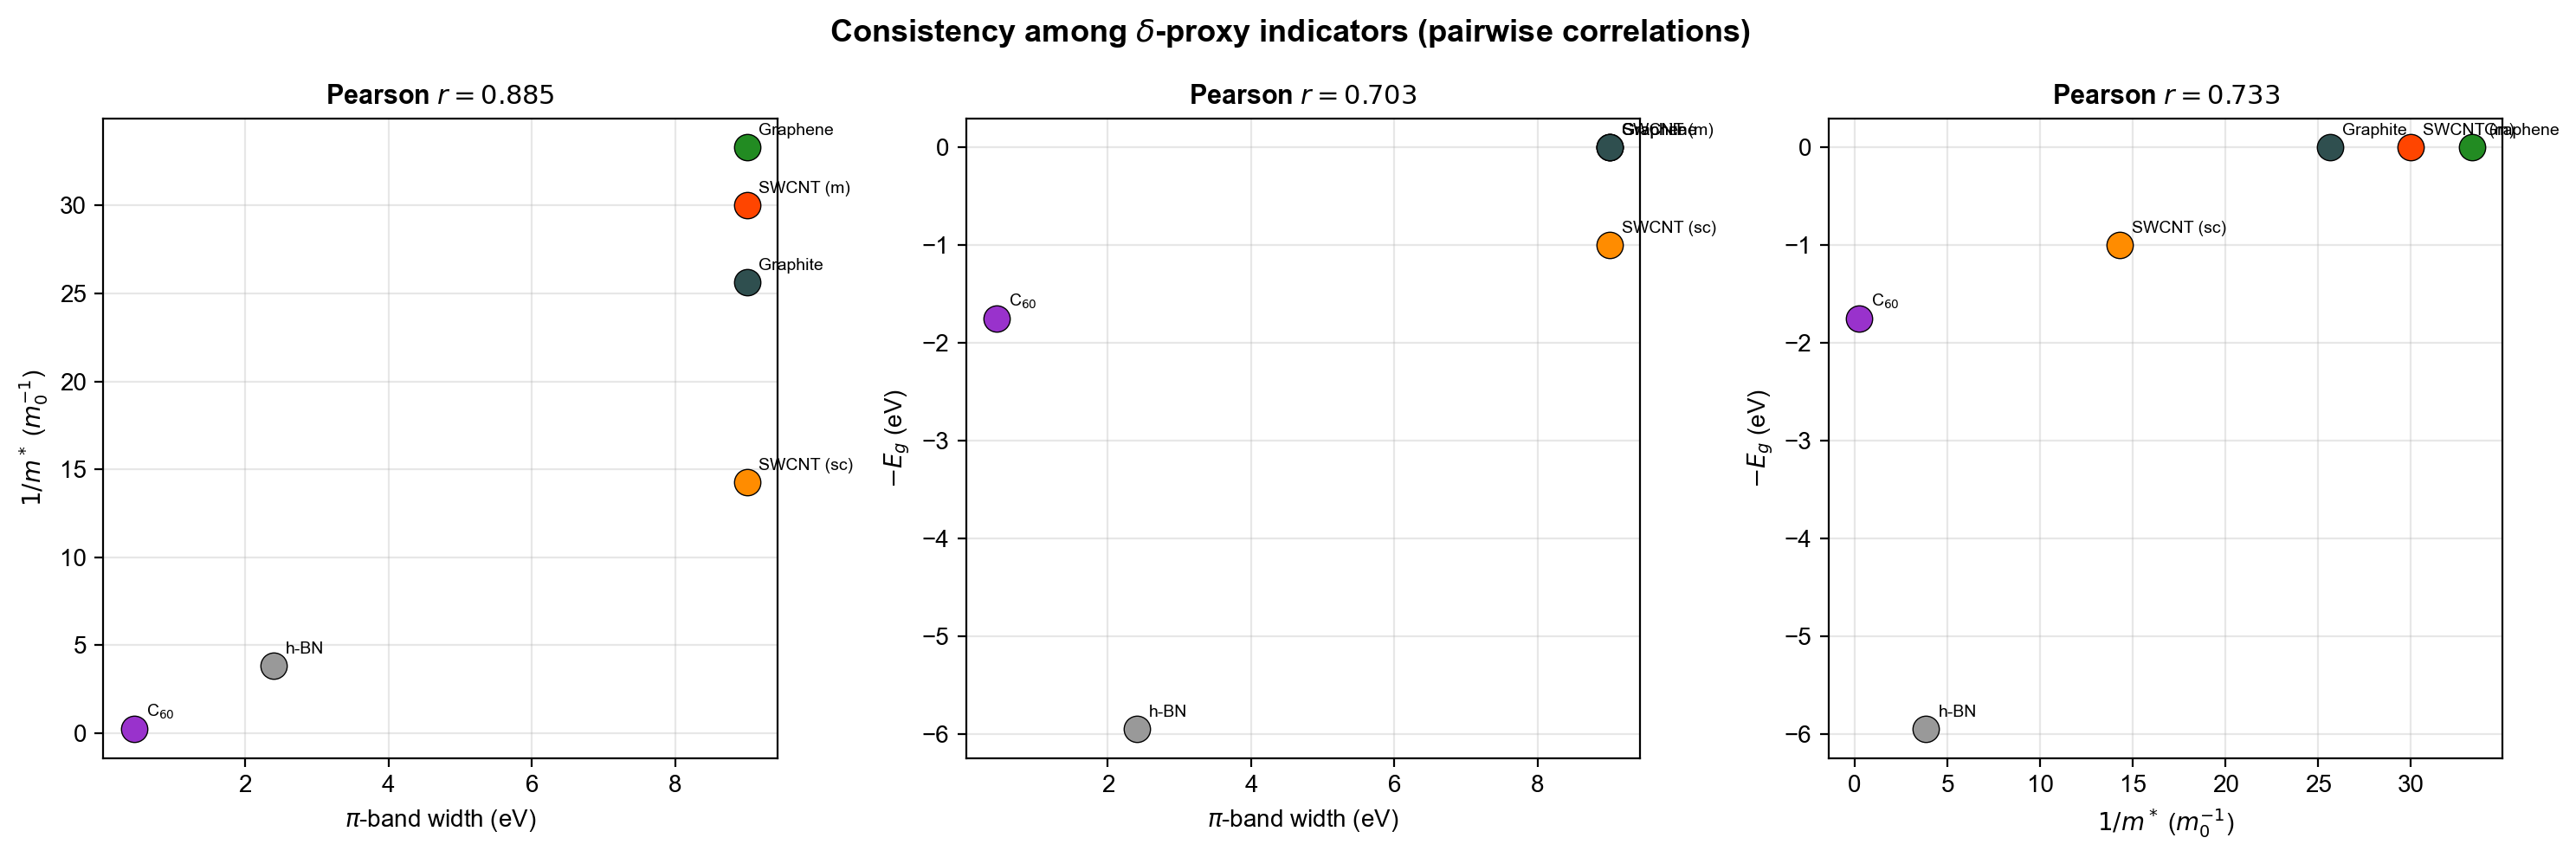
\includegraphics[width=\columnwidth]{fig4_indicator_consistency}
  \caption{Pairwise scatter plots among the three $\delta$-proxy
    indicators, with Pearson and Spearman correlation coefficients.}
  \label{fig:consistency}
\end{figure}

\subsection{$E_g \times D_\mathrm{eff}$ optical-response map}

Figure~\ref{fig:Eg_Deff} shows all seven materials plotted in
$E_g$--$D_\mathrm{eff}$ space, with the decision-tree classification
boundaries overlaid. Each material falls unambiguously into the correct
optical-response region.

\begin{figure}[t]
  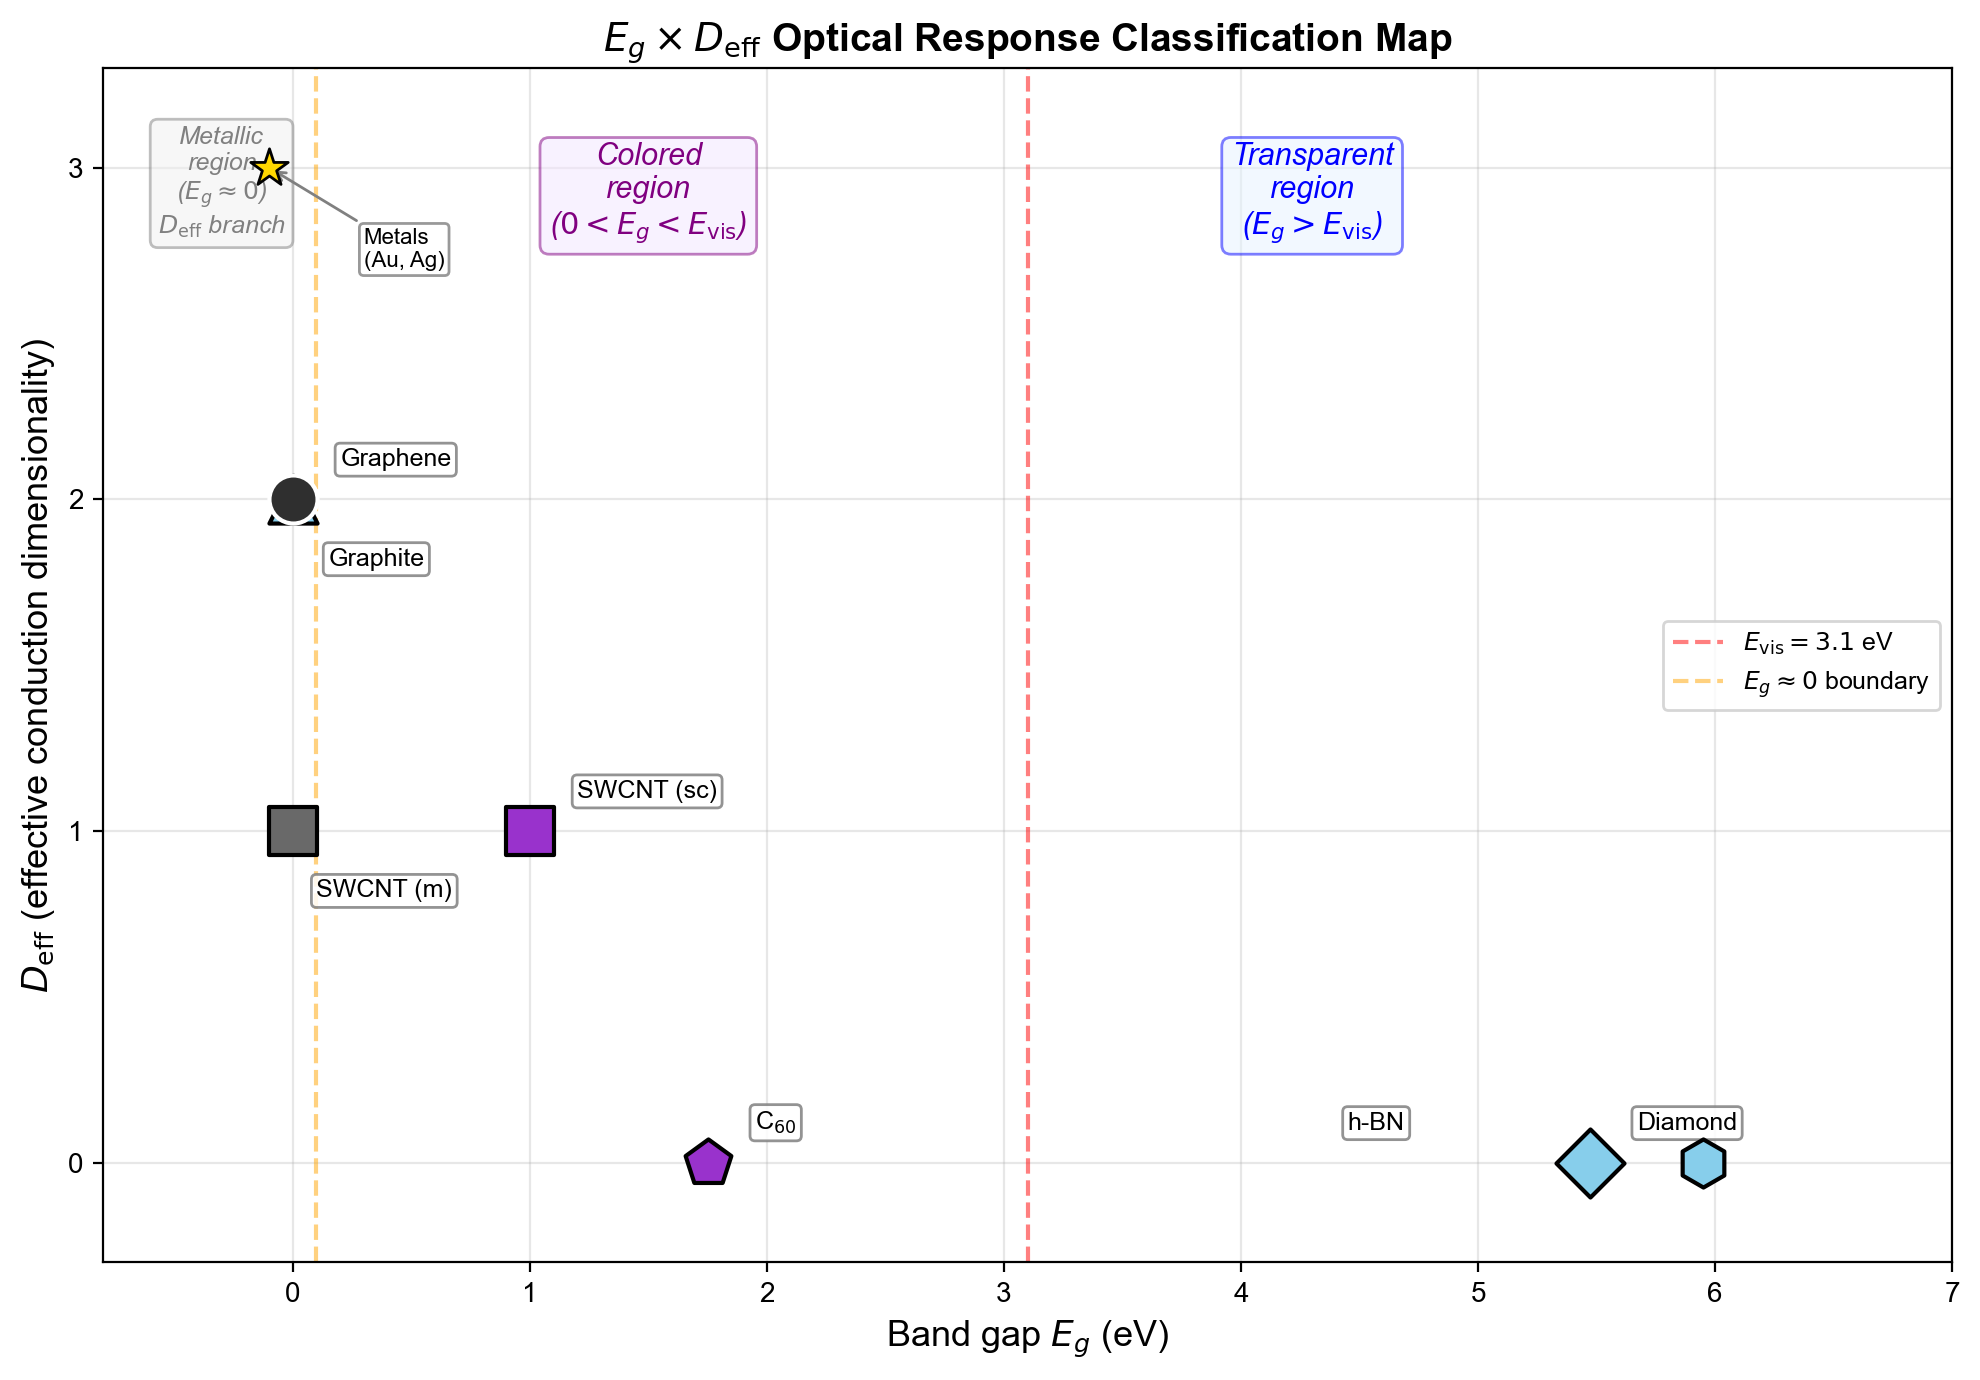
\includegraphics[width=\columnwidth]{fig6_Eg_Deff_classification}
  \caption{Optical-response classification map in
    $E_g$--$D_\mathrm{eff}$ space. Shaded regions correspond to
    decision-tree categories (Sec.~\ref{sec:tree}). All seven materials
    are classified correctly.}
  \label{fig:Eg_Deff}
\end{figure}

\subsection{Classification accuracy}

\begin{table}[h]
\caption{Decision-tree classification results.}
\label{tab:classification}
\begin{ruledtabular}
\begin{tabular}{lccllc}
  Material & $E_g$ (eV) & $D_\mathrm{eff}$ & Predicted & Observed & \\
  \hline
  Diamond      & 5.47 & 0 & Transparent & Transparent & \checkmark \\
  C$_{60}$     & 1.75 & 0 & Colored     & Colored     & \checkmark \\
  SWCNT (sc)   & 1.0  & 1 & Colored     & Colored     & \checkmark \\
  SWCNT (m)    & 0    & 1 & Black$-$luster & Black$-$luster & \checkmark \\
  Graphene     & 0    & 2 & Transparent$^*$ & Transparent & \checkmark \\
  Graphite     & 0    & 2 & Black$+$gloss & Black$+$gloss & \checkmark \\
  h-BN         & 5.95 & 0 & Transparent & Transparent & \checkmark \\
\end{tabular}
\end{ruledtabular}
\end{table}

\noindent Classification accuracy: 7/7 = 100\%.

$^*$Single-layer graphene absorbs only $\pi\alpha \approx 2.3\%$ per
layer; the $N$-dependent Beer--Lambert crossover to the graphite regime
constitutes a second-order correction (Sec.~\ref{sec:framework}).

\subsection{h-BN as a control system}
\label{sec:hBN}

h-BN shares the layered sp$^2$ network topology of graphite, so one
might expect $D_\mathrm{eff} = 2$. However, the electronegativity
difference between B and N breaks the sublattice (spatial-inversion)
symmetry: the $\pi$ electrons localize on nitrogen sites, reducing
$W_\pi$ from 9~eV (graphite) to 2.4~eV and opening a gap of 5.95~eV.
In the language of the present framework, the symmetry-breaking
potential localizes the $\pi$ electrons, \emph{lowering}~$\delta$. Since
$E_g$ far exceeds the visible-energy window, $D_\mathrm{eff} = 0$
despite the 2D crystal structure.

This demonstrates two key points: (i)~$D_\mathrm{eff}$ is not
reducible to crystallographic dimensionality, and (ii)~$\delta$ is an
independent variable whose variation can flip the optical response
from black to transparent within the same structural family.

\subsection{Tight-binding simulation results}

\begin{figure}[t]
  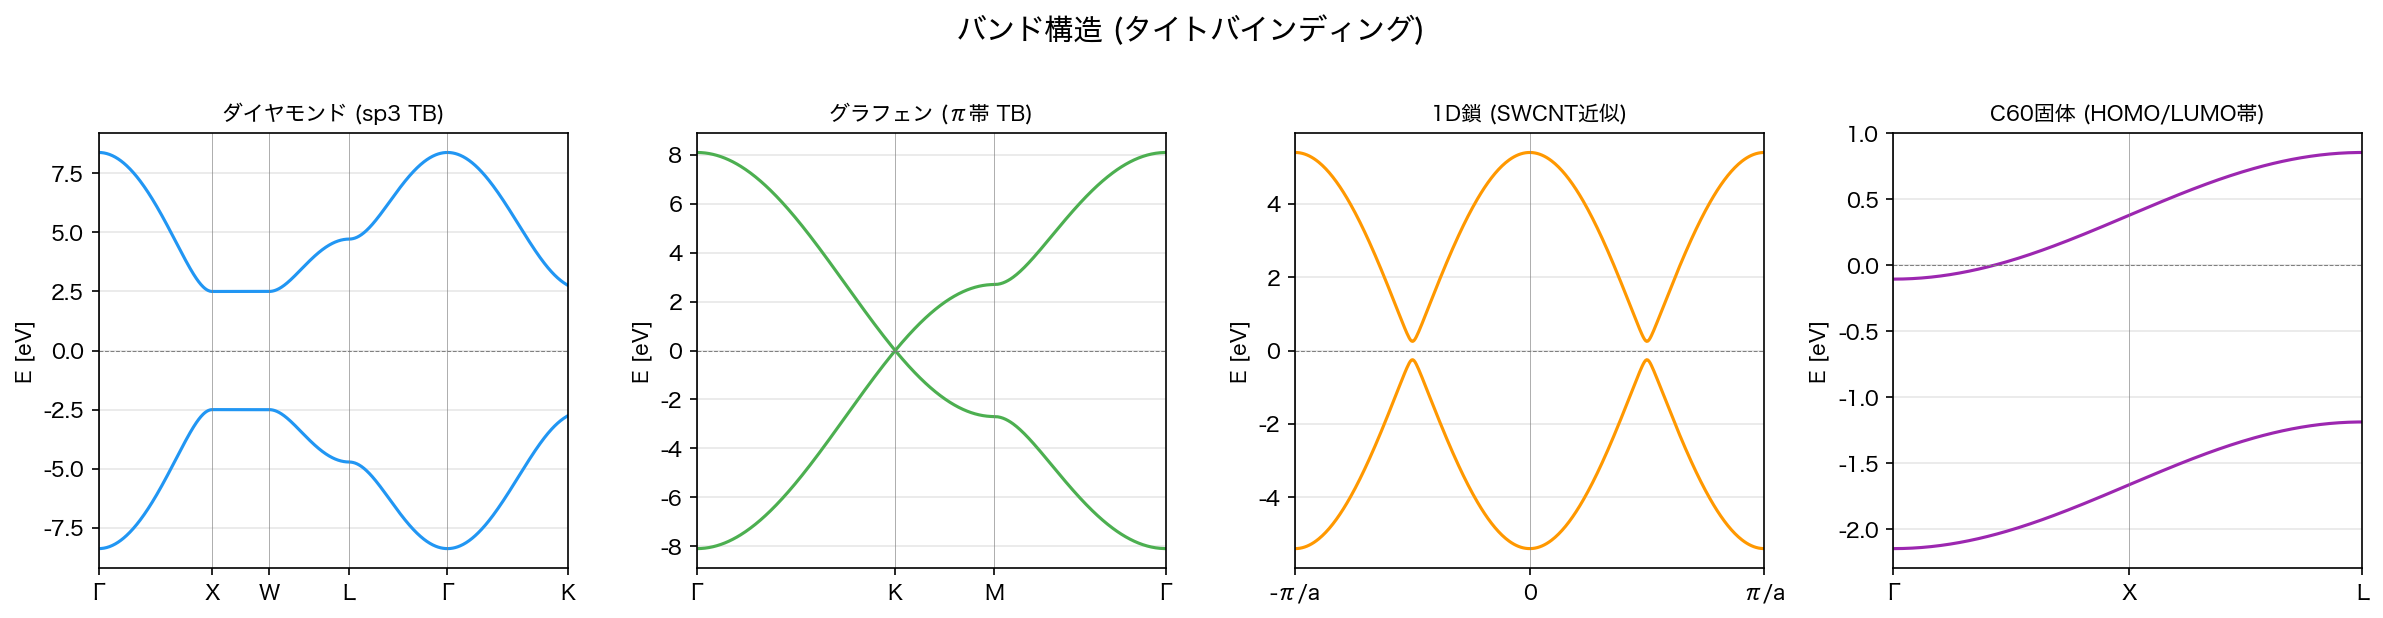
\includegraphics[width=\columnwidth]{fig_a_bandstructure}
  \caption{Tight-binding band structures for four model systems:
    diamond, graphene, 1D chain (SWCNT proxy), and C$_{60}$ cluster.}
  \label{fig:bands}
\end{figure}

\begin{figure}[t]
  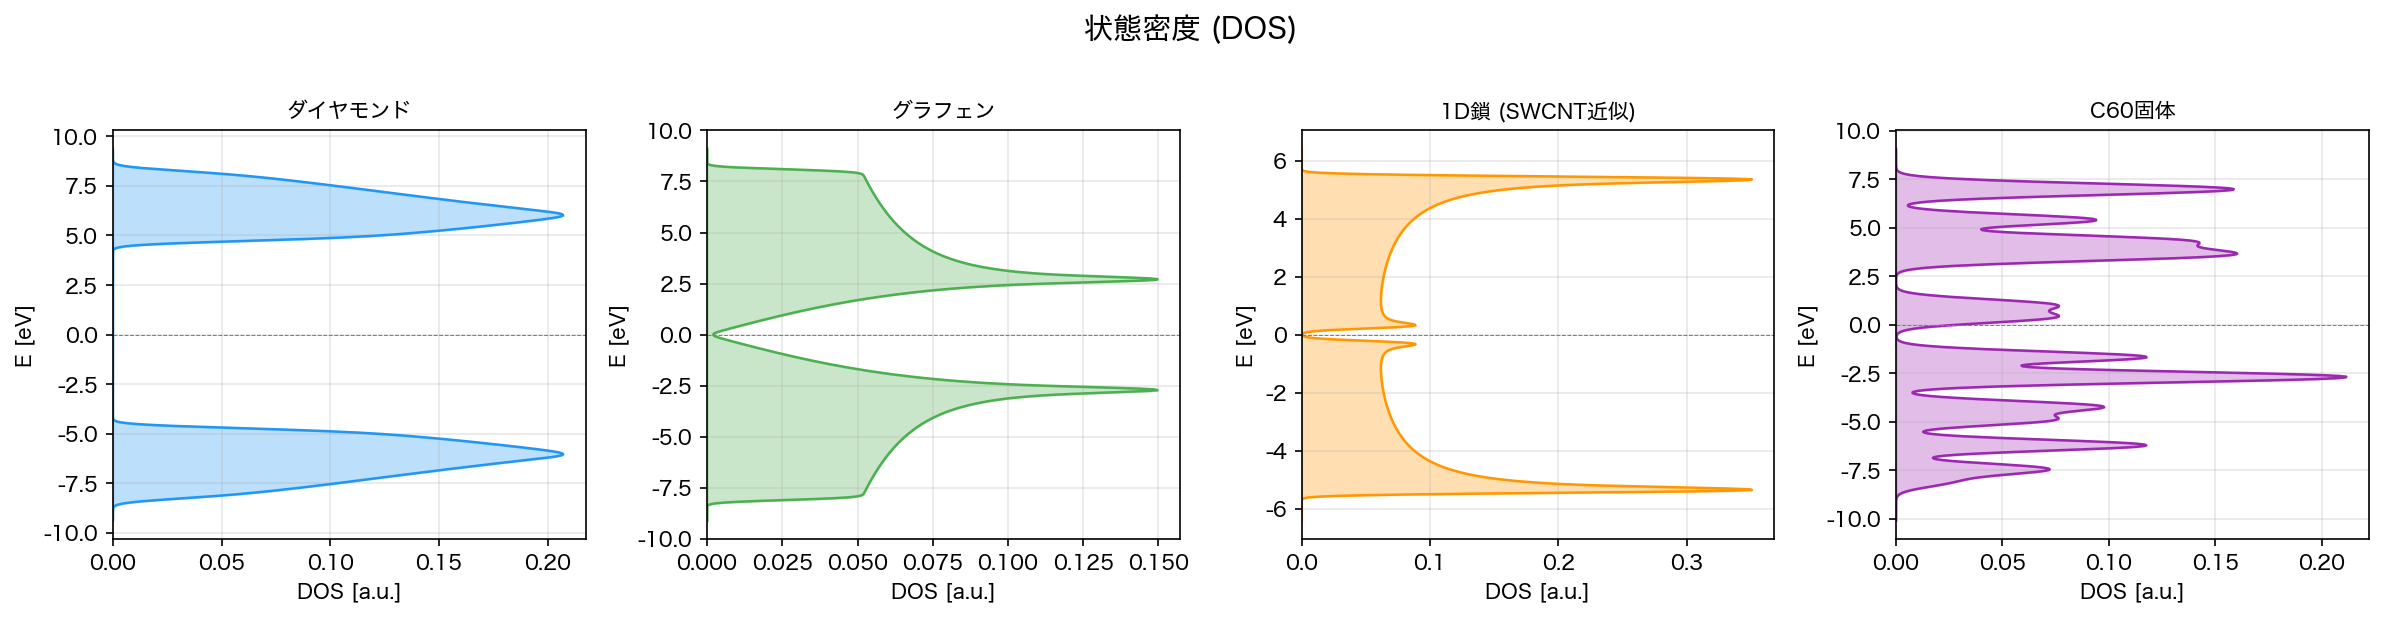
\includegraphics[width=\columnwidth]{fig_b_dos}
  \caption{Density of states for the four model systems.
    Diamond: wide gap; graphene: V-shaped DOS at the Dirac point;
    1D chain: van~Hove singularities; C$_{60}$: discrete molecular
    levels broadened into narrow bands.}
  \label{fig:dos}
\end{figure}

\subsubsection{$D_\mathrm{eff}$ from the velocity tensor}

The effective rank of $\langle v_\alpha v_\beta \rangle$ was computed
for each system from the full Slater--Koster (diamond, graphene) or
$\pi$-band (1D chain) Hamiltonian. The results---diamond: 3.00,
graphene: 2.00, 1D chain: 1.00, C$_{60}$: 0.00---reproduce the
expected integer values exactly, confirming that $D_\mathrm{eff}$ as
defined in Eq.~\eqref{eq:Deff} is computable from band structure
without ambiguity.

\subsubsection{Optical conductivity and consistency with
  $\varepsilon(\omega)$}

The Kubo formula applied to the same Hamiltonian yields the optical
conductivity $\sigma(\omega)$, from which $\varepsilon_2(\omega)$ and
the normal-incidence reflectivity $R(\omega)$ follow. For graphene,
the low-energy conductivity correctly reproduces the universal value
$\sigma_0 = \pi e^2 / 2h$ ($\sigma/\sigma_0 = 1.000$). The
full-orbital model yields visible-range reflectivities of
$R_\mathrm{vis} \approx 0.34$ for graphene/graphite and
$R_\mathrm{vis} \approx 0.31$ for diamond, in qualitative agreement
with experimental values ($\sim$0.25--0.30 and $\sim$0.17,
respectively). Diamond's overestimate is attributable to the well-known
band-gap underestimation of the Slater--Koster parametrization.

\begin{figure}[t]
  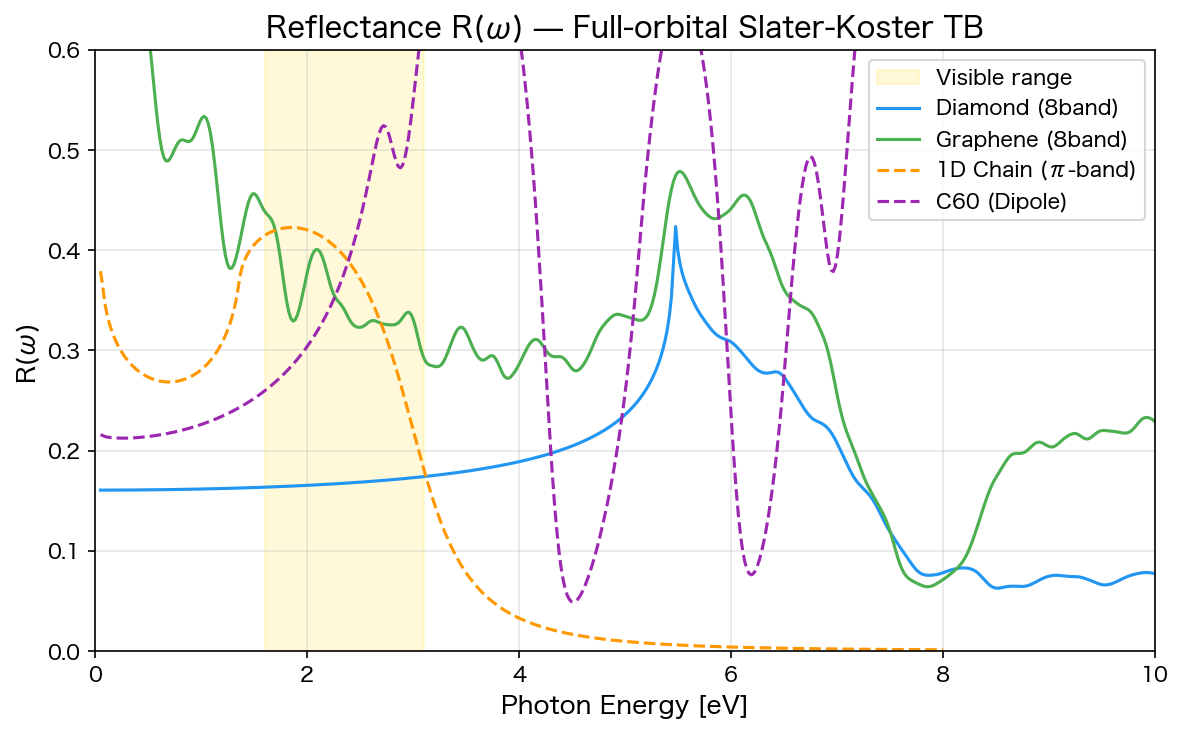
\includegraphics[width=\columnwidth]{fig_e_reflectivity}
  \caption{Reflectivity $R(\omega)$ computed from the Kubo formula for
    all four model systems. The yellow shaded region marks the visible
    range (1.6--3.1~eV). Diamond and graphene use the full
    Slater--Koster 8-band model; the 1D chain and C$_{60}$ use
    $\pi$-band and dipole models, respectively.}
  \label{fig:reflectivity}
\end{figure}

The key observation is that $D_\mathrm{eff}$ and
$\varepsilon(\omega)$ are derived from the \emph{same} band
structure and are mutually consistent in the solid-state regime. This
consistency provides the foundation for extending $D_\mathrm{eff}$ to
systems where $\varepsilon(\omega)$ is difficult to define---notably
liquids and non-periodic interfaces---as a reliable classification
variable.

\subsubsection{$\delta$--$E_g$ correlation}

The IPR-based $\delta$ correlates inversely with $E_g$ across the four
model systems (Pearson $r = -0.86$; Fig.~\ref{fig:TB_corr}).

\begin{figure}[t]
  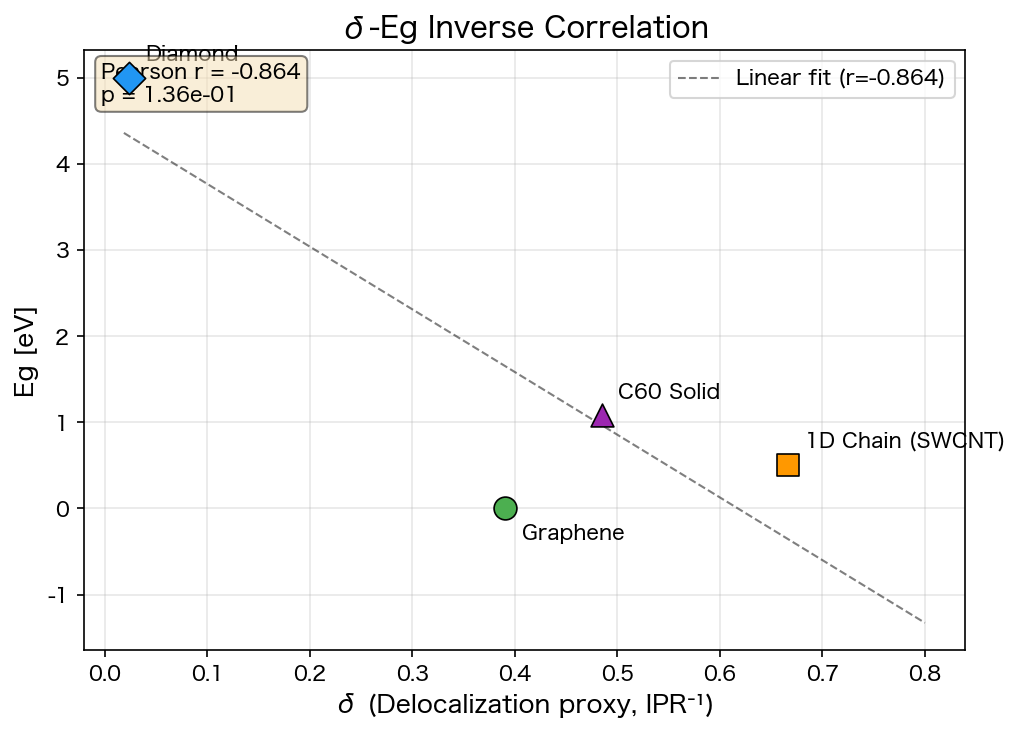
\includegraphics[width=\columnwidth]{fig_c_delta_Eg_correlation}
  \caption{IPR-based delocalization index $\delta$ versus band gap
    $E_g$ from tight-binding calculations ($r = -0.86$).}
  \label{fig:TB_corr}
\end{figure}

\subsection{$\delta \times D_\mathrm{eff}$ maps}

\begin{figure}[t]
  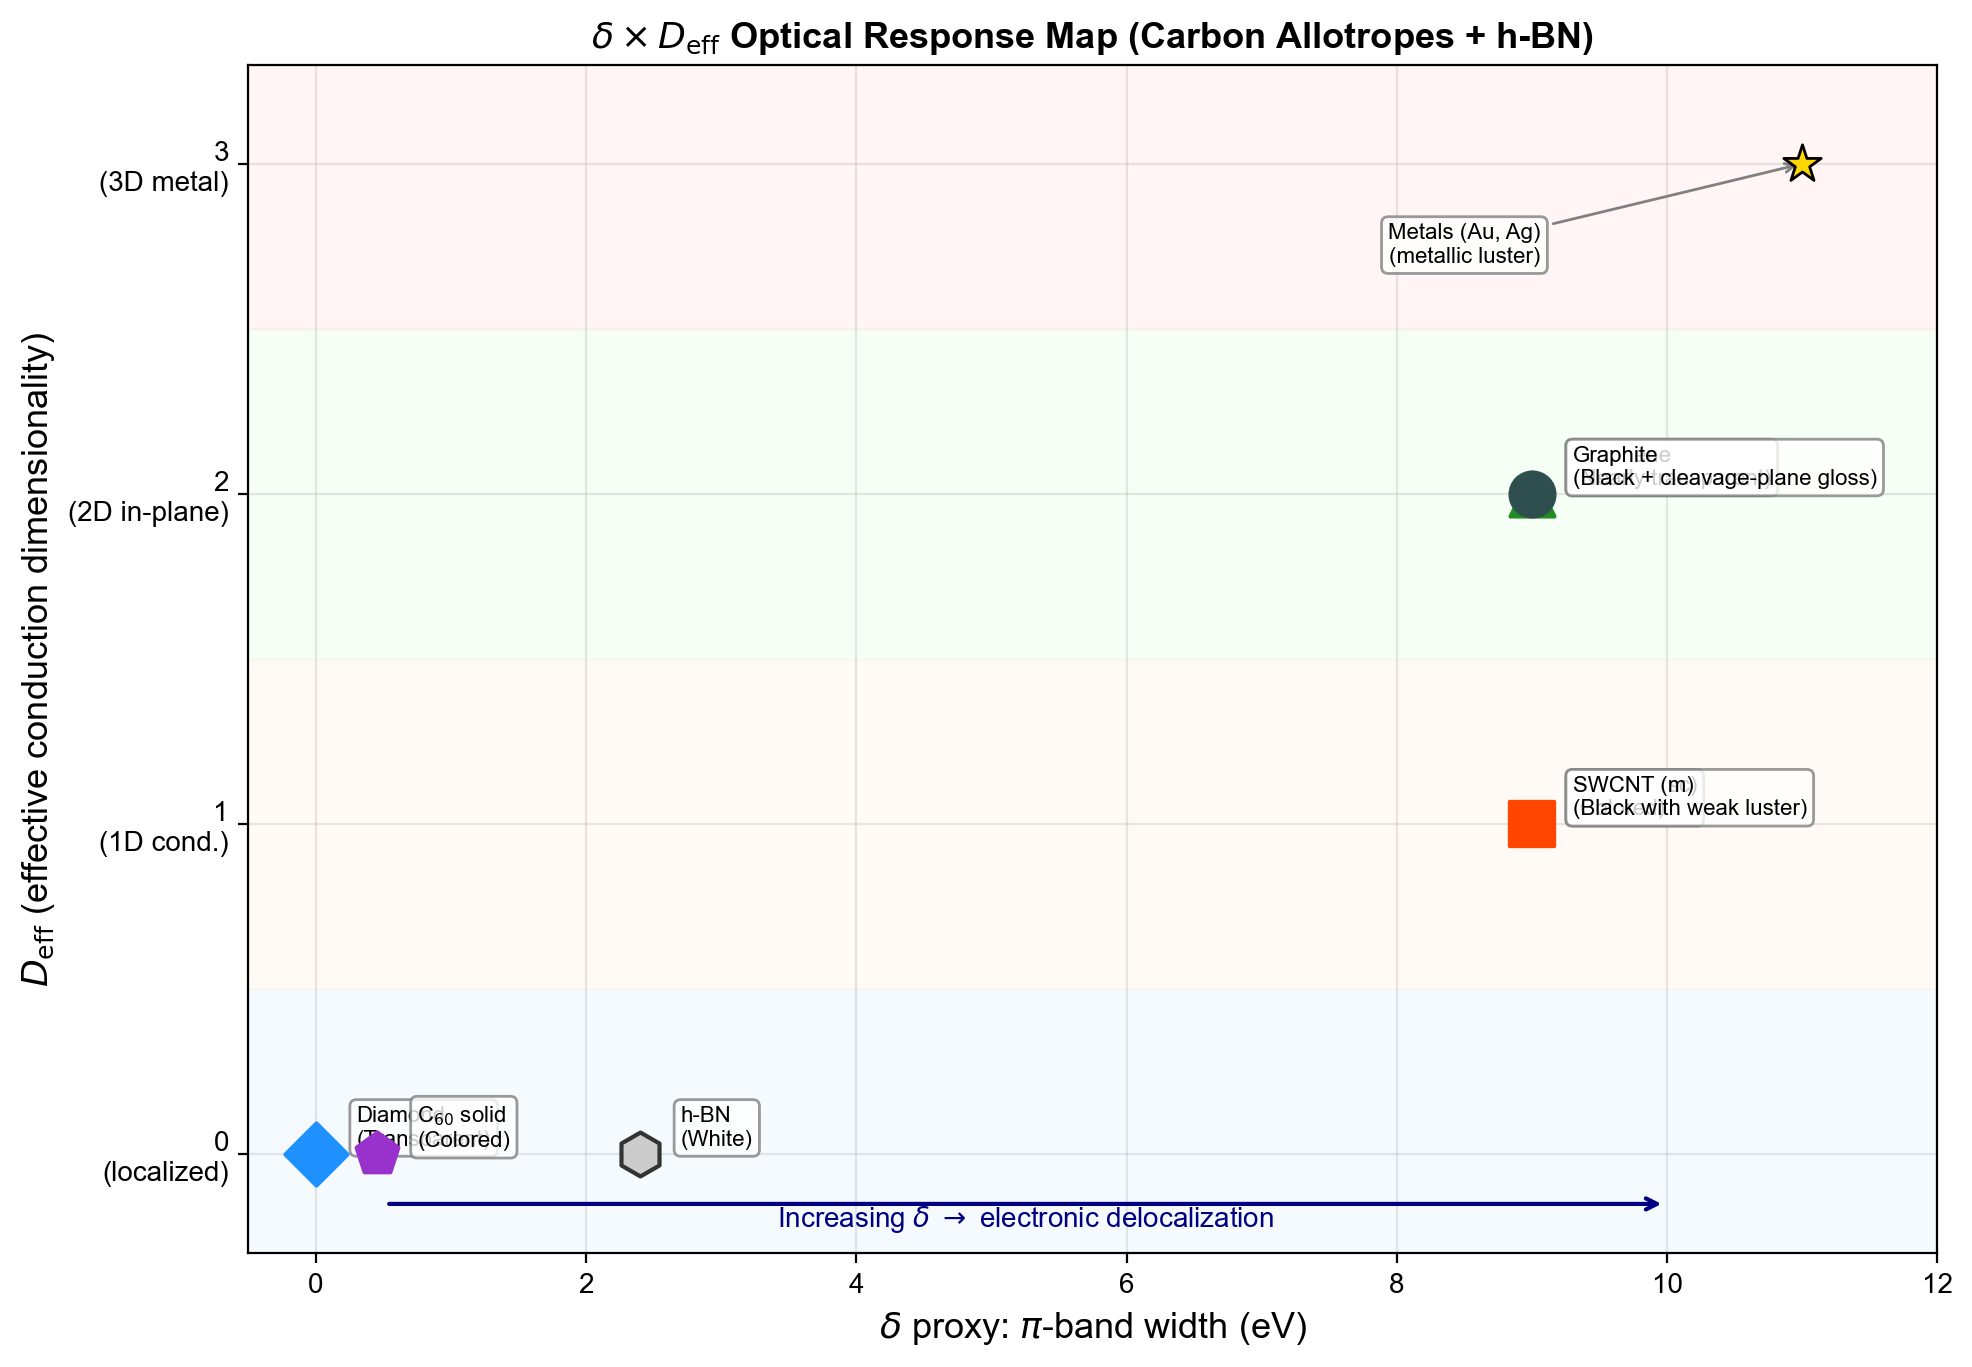
\includegraphics[width=\columnwidth]{fig1_delta_deff_map}
  \caption{$\delta$ ($\pi$-band width) vs.\ $D_\mathrm{eff}$ map.
    Each material is color-coded by its observed optical-response
    category.}
  \label{fig:delta_map}
\end{figure}

\begin{figure}[t]
  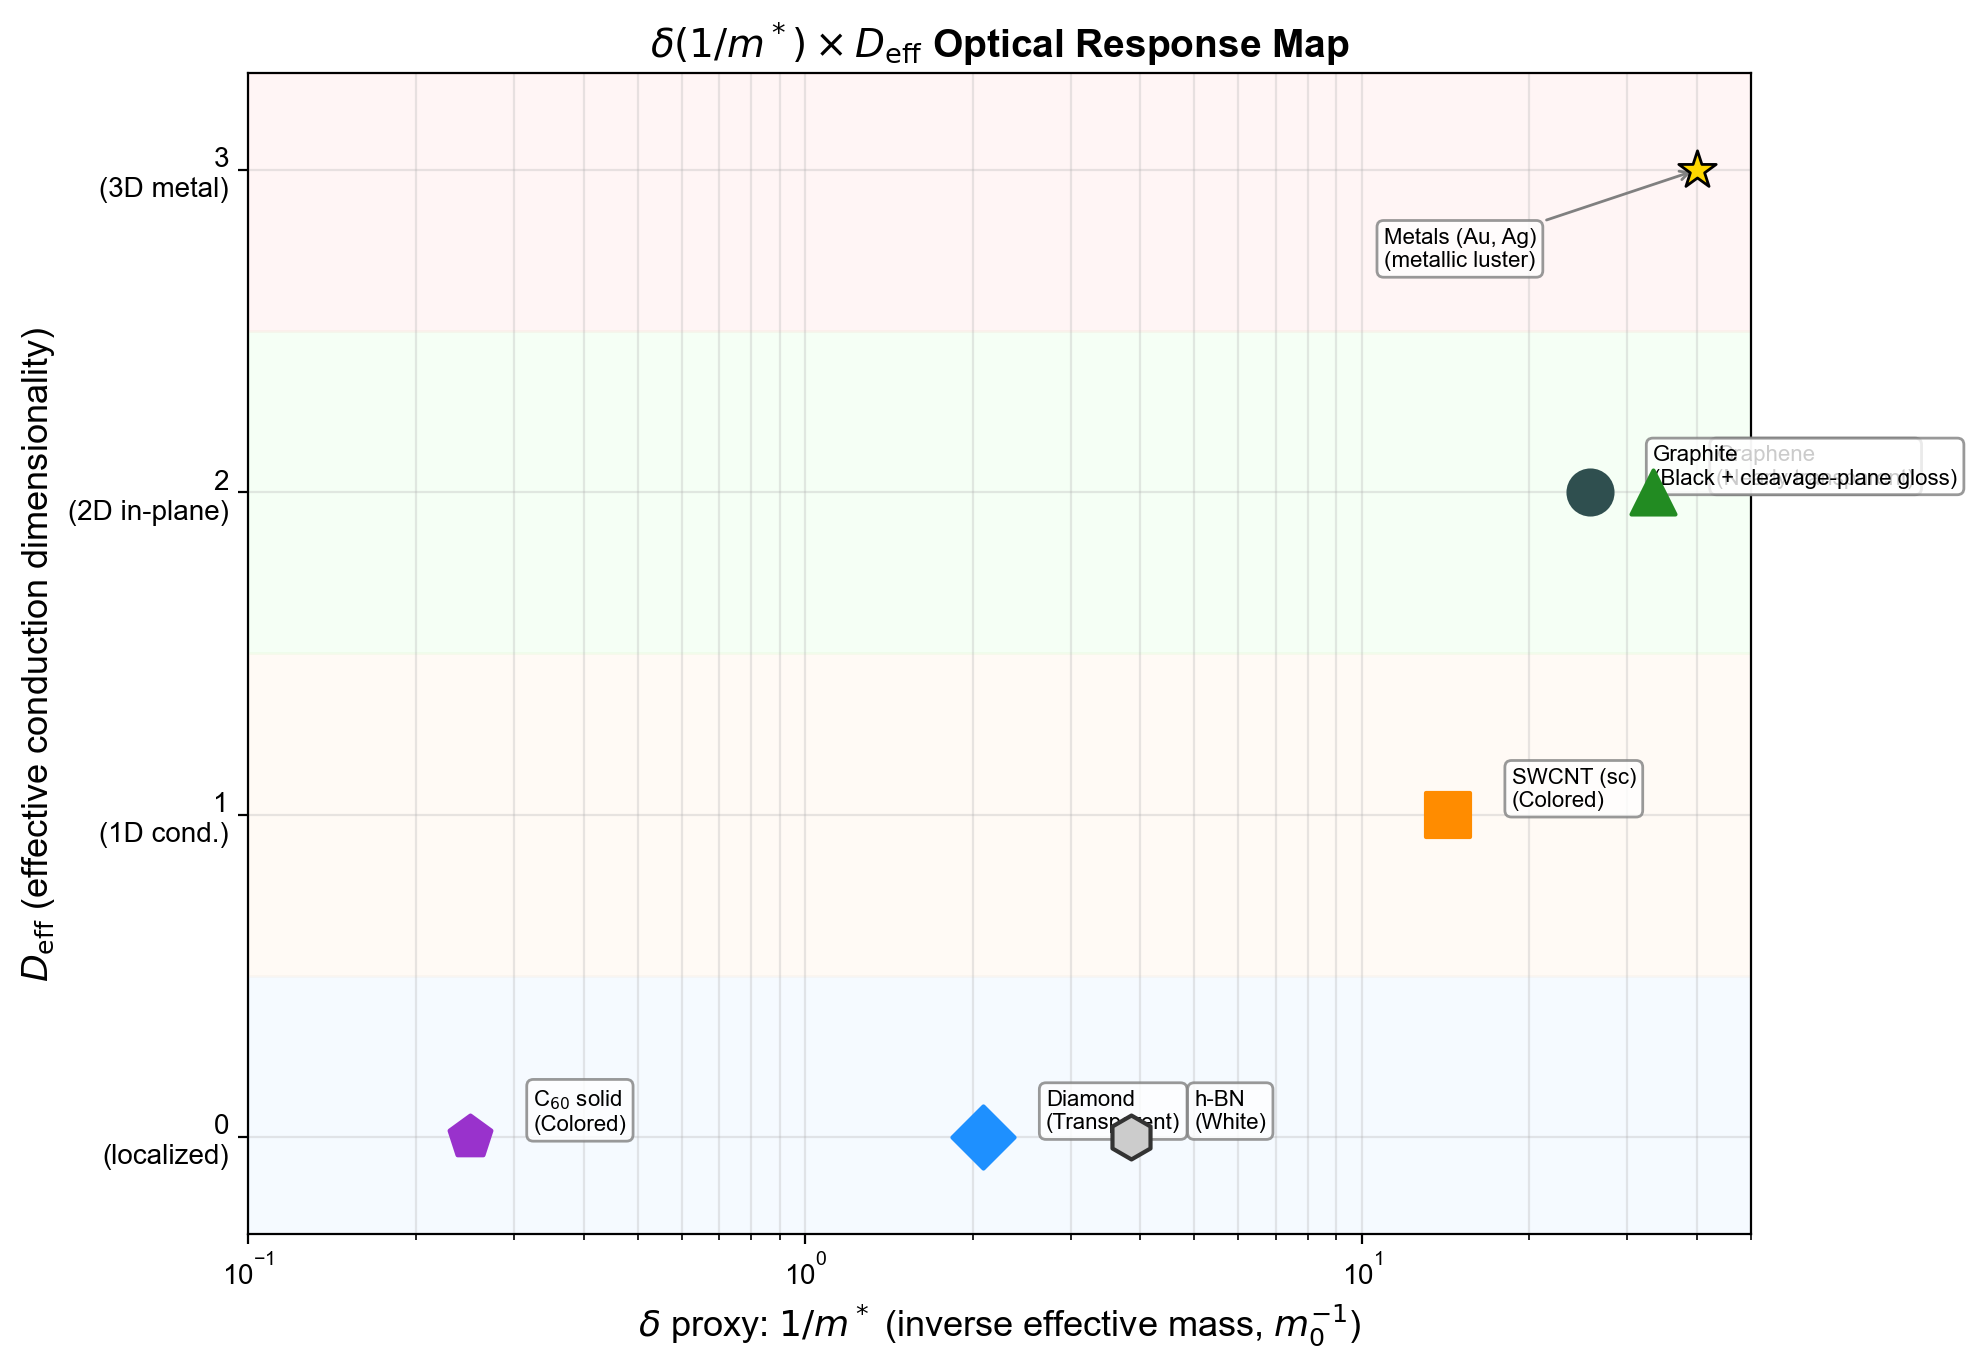
\includegraphics[width=\columnwidth]{fig3_invmass_deff_map}
  \caption{$\delta$ (inverse effective mass, log scale) vs.\
    $D_\mathrm{eff}$ map. The ordering of materials along the
    $\delta$ axis is consistent with Fig.~\ref{fig:delta_map}.}
  \label{fig:invmass_map}
\end{figure}

\begin{figure}[t]
  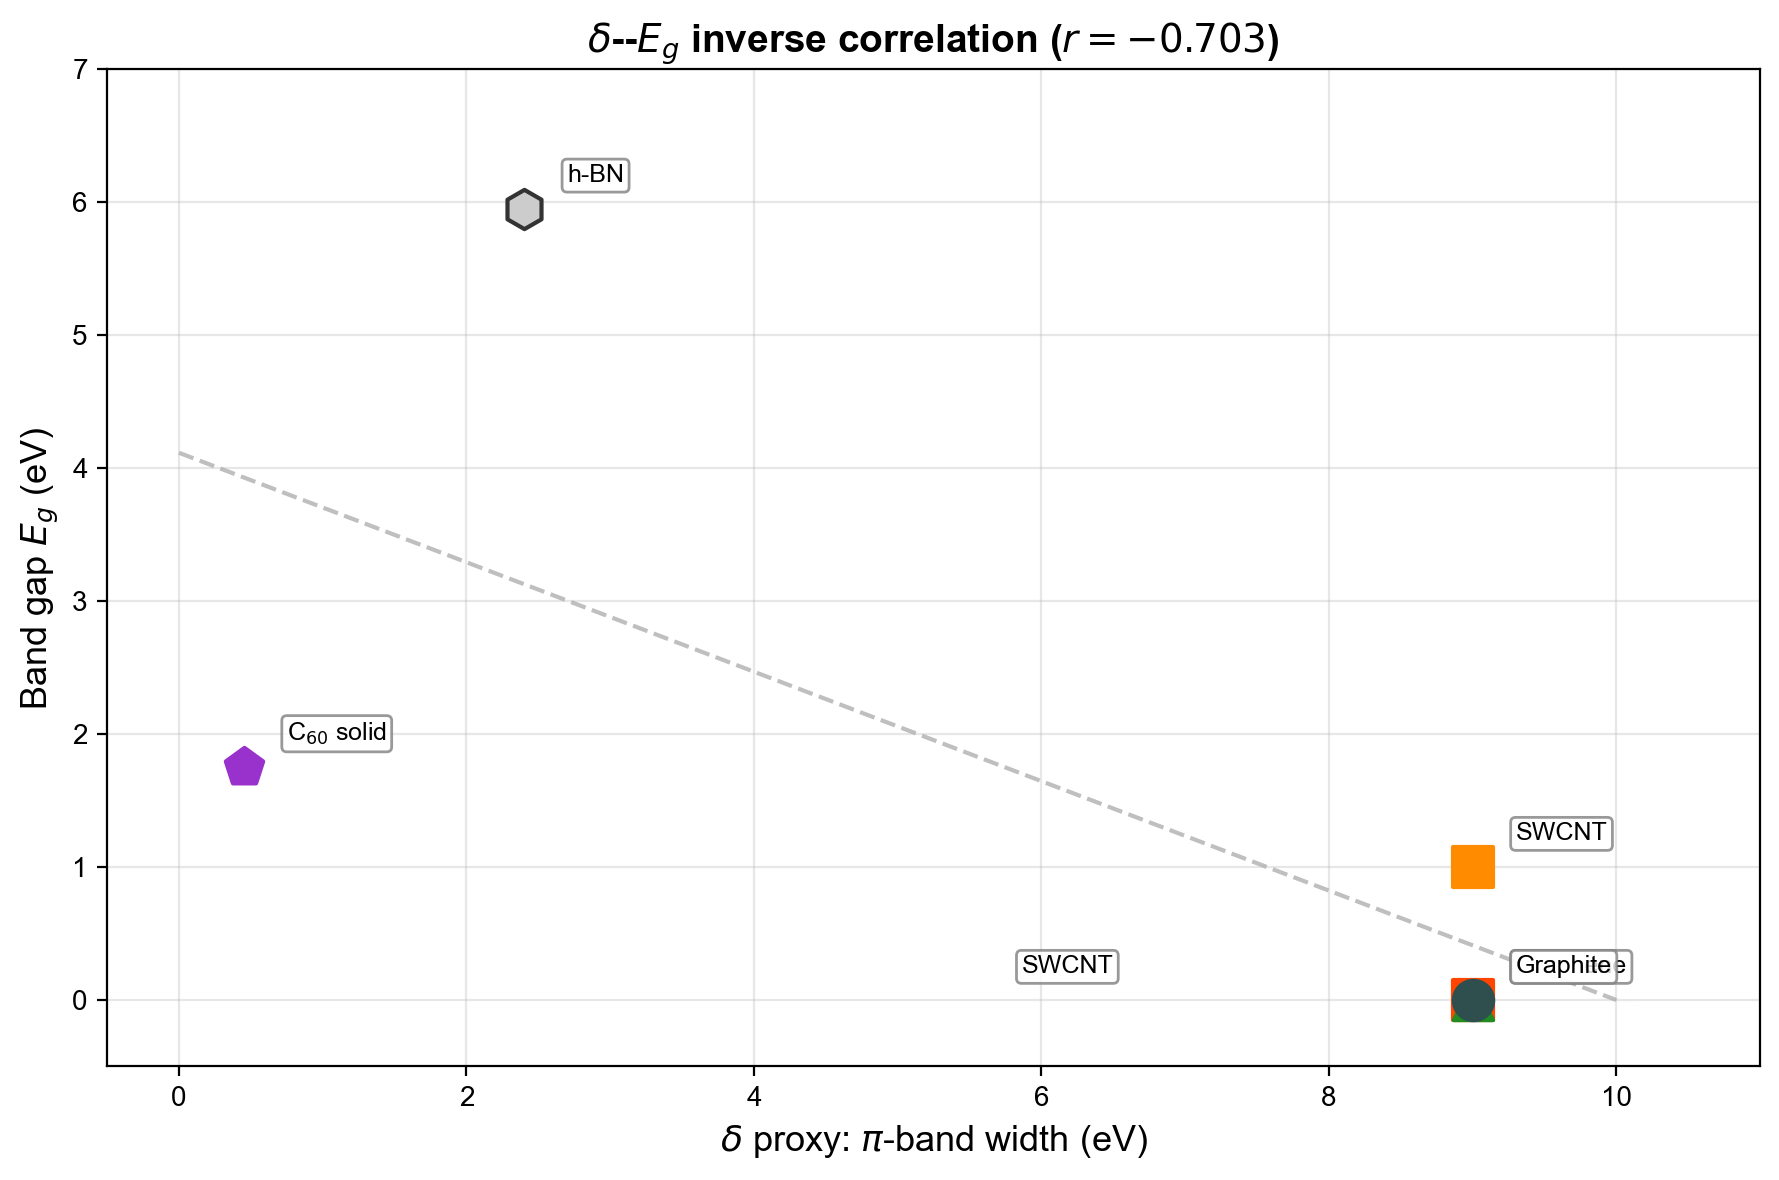
\includegraphics[width=\columnwidth]{fig2_delta_bandgap_correlation}
  \caption{$\delta$ ($\pi$-band width) vs.\ band gap $E_g$
    from published data ($r = -0.703$).}
  \label{fig:delta_Eg}
\end{figure}

% =====================================================================
\section{Discussion}
\label{sec:discussion}
% =====================================================================

\subsection{$\delta$ as the coherence-preservation condition}

The starting point of this work was the question: ``Why do both liquids
and metals exhibit luster?'' Luster is the preservation of photon phase
coherence at an interface, and its condition reduces to the freedom of
constituent particles~($\delta$).

The solid-state verification presented here demonstrates that electronic
delocalization~$\delta$ is a fundamental variable governing optical
response. This result is consistent with the broader hypothesis that
$\delta$---whether electronic or nuclear---universally determines
whether an interface acts as a coherent or incoherent quantum barrier.

\subsection{Role of $\delta$, $E_g$, and $D_\mathrm{eff}$}

The contribution of this work is the introduction of $D_\mathrm{eff}$
as a second classification axis alongside~$E_g$:
\begin{itemize}
  \item $E_g$ determines \emph{at which energy} the optical response
    occurs.
  \item $D_\mathrm{eff}$ determines \emph{in how many spatial
    directions} the response is strong, resolving degeneracies that
    $E_g$ alone cannot lift (e.g., graphite vs.\ metals at
    $E_g \approx 0$).
  \item The concept of particle freedom~($\delta$) motivated the
    introduction of $D_\mathrm{eff}$; $\delta$ itself is not used as
    a classification variable in this work. Its independent
    verification---particularly through extension to liquid and
    interfacial systems where $E_g$ is ill-defined---is a natural
    target for future study.
\end{itemize}

\subsection{Relation to existing theories}

\begin{table}[h]
\caption{Relation of the $\delta \times D_\mathrm{eff}$ framework to
  established theories.}
\label{tab:existing}
\begin{ruledtabular}
\begin{tabular}{ll}
  Existing theory & Relation to present framework \\
  \hline
  Drude model & Special case: $D_\mathrm{eff} = 3$, $\delta$ high \\
  Band theory & $E_g$ is one axis; $D_\mathrm{eff}$ adds the second \\
  Crystal-field theory & $10Dq \approx$ local modulation of $\delta$ \\
  Fresnel optics & Presupposes uniform $\varepsilon(\omega)$; \\
   & this uniformity itself depends on $\delta$ \\
\end{tabular}
\end{ruledtabular}
\end{table}

\subsection{h-BN and the breaking of sublattice symmetry}
\label{sec:hBN_discussion}

The dramatic optical contrast between graphite (black) and h-BN (white)
is conventionally attributed to the sublattice symmetry breaking caused
by the B--N electronegativity difference. In the present framework, this
symmetry breaking has a direct translation: the staggered on-site
potential~$\Delta$ localizes the $\pi$ electrons onto nitrogen sites,
\emph{reducing}~$\delta$. Quantitatively, the tight-binding model for a
honeycomb lattice with sublattice potential~$\Delta$ gives
$E_g = 2\Delta$ and reduces the effective bandwidth available for
optical transitions. The two descriptions---symmetry breaking (band
theory) and $\delta$ reduction (present framework)---are mathematically
equivalent for bipartite lattices, confirming that the $\delta$~language
is consistent with, and not in conflict with, the standard solid-state
picture.

\subsection{Prior work}

To our knowledge, no prior publication has:
\begin{enumerate}
  \item Constructed an explicit decision tree classifying macroscopic
    optical response using band gap and effective conduction
    dimensionality.
  \item Defined $D_\mathrm{eff}$ as a formal classification variable
    distinct from crystallographic dimensionality.
  \item Systematically benchmarked optical-response classification
    across carbon allotropes using two variables.
  \item Unified multiple delocalization proxies under a single
    overarching index $\delta$ and tested their mutual consistency.
\end{enumerate}

The closest related work is Shi and Yao \textit{et al.}\ (Carbon, 2020),
who classified carbon allotropes as metallic, semiconducting, or
insulating using density and bond angle---but their framework addresses
the \emph{electronic phase}, not the \emph{optical appearance}, and
lacks a dimensionality variable.

\subsection{Limitations}

\begin{enumerate}
  \item The verification is limited to seven materials (five carbon
    allotropes + h-BN + metal reference).
  \item The operational definition of $\delta$ is not unique; however,
    the agreement among three independent proxies provides empirical
    support for its existence.
  \item The graphene--graphite crossover requires thickness~$N$ as
    an additional parameter (Beer--Lambert regime).
  \item The coherence-preservation hypothesis for luster is not
    directly tested in this work; only its solid-state electronic
    consequence ($\delta \times D_\mathrm{eff}$ classification) is
    verified.
\end{enumerate}

\subsection{Outlook}

\begin{itemize}
  \item \textbf{Liquids}: The nuclear delocalization
    $\delta_\mathrm{nuc}$ and its role in interface self-smoothing.
    The solid-to-liquid reflectivity jump of gallium (50\% $\to$ 90\%)
    is a direct test case.
  \item \textbf{Interfaces and catalysis}: Whether the discontinuity
    of $\delta$ at heterojunctions governs charge-transfer rates.
    Connection to the d-band center theory of catalytic activity.
  \item \textbf{First-principles $\delta$}: Systematic DFT calculation
    of IPR, Wannier spreads, and optical conductivity to place $\delta$
    on a quantitative, non-proxy footing.
  \item \textbf{Inverse design}: Given a target optical response,
    invert $\delta \times D_\mathrm{eff}$ to identify candidate
    structures.
  \item \textbf{Cross-element validation}: Transition-metal oxides,
    organic semiconductors, and perovskites.
\end{itemize}

% =====================================================================
\section{Conclusion}
\label{sec:conclusion}
% =====================================================================

Luster is the preservation of photon phase coherence at an interface.
We propose that its microscopic condition reduces to the freedom of
constituent particles, quantified by a delocalization index~$\delta$.

As a proof of concept, we constructed a two-variable phenomenological
framework ($\delta_\mathrm{elec}$, $D_\mathrm{eff}$) and tested it on
five carbon allotropes and an h-BN control. A decision tree based on
$E_g$ and $D_\mathrm{eff}$ classifies all seven materials into the
correct optical-response category (transparent, colored, black, or
lustrous) with 100\% accuracy. Three independent $\delta$-proxy
indicators show statistically significant pairwise correlations,
supporting the existence of an overarching delocalization
variable~$\delta$.

The framework does not replace band-gap theory; it extends it by
adding $D_\mathrm{eff}$ as a second classification axis.
$E_g$ determines \emph{at which energy} the response occurs, while
$D_\mathrm{eff}$ determines its \emph{directionality}. The concept of
particle freedom~($\delta$) that motivated $D_\mathrm{eff}$ remains to
be independently verified; extension to liquid, interfacial, and
cross-element systems---where $E_g$ is ill-defined but $\delta$ may
still apply---is proposed as a target for future work.

\begin{acknowledgments}
The initial inspiration for this work arose from observing the luster
of water at a public bathhouse (\textit{sent\=o}).
\end{acknowledgments}

\section*{Use of AI-assisted tools}

The conceptual framework---the hypothesis that particle freedom
($\delta$) governs photon coherence preservation at interfaces, the
definitions of $\delta$ and $D_\mathrm{eff}$, and the decision-tree
classification---was conceived entirely by the author.

The experimental design, literature data collection, statistical
verification, tight-binding simulation code, and manuscript drafting
were conducted with substantial assistance from large language models
(Claude, Anthropic; GPT-4o, OpenAI; Grok, xAI). Specifically:

\begin{itemize}
  \item \textbf{Data collection}: Published values of $\pi$-band
    widths, effective masses, band gaps, and optical properties were
    gathered from the literature with AI assistance. All values were
    cross-checked by the author against primary sources.
  \item \textbf{Simulation}: The tight-binding proof-of-concept code
    (\texttt{delocalization\_optics\_v2.py}) was developed with AI
    assistance. The code and its outputs were reviewed and validated
    by the author.
  \item \textbf{Statistical analysis}: Correlation analyses and
    classification tests were performed with AI assistance and
    independently verified by the author.
  \item \textbf{Manuscript}: The English draft was prepared with AI
    assistance based on the author's Japanese notes and structural
    outline.
  \item \textbf{Peer review simulation}: Pre-submission review
    feedback was solicited from multiple AI systems to identify
    potential weaknesses and strengthen the manuscript.
\end{itemize}

\noindent The author assumes full responsibility for the scientific
content, interpretation, and conclusions presented in this work.

\bibliography{references}

\end{document}
